\documentclass[12pt, a4paper]{article}

% חבילות לתמיכה מושלמת בעברית (יש לקמפל באמצעות XeLaTeX ב-Overleaf)
\usepackage{fontspec}
\usepackage{polyglossia}
\setdefaultlanguage{hebrew}
\setotherlanguage{english}

% הגדרת גופן בהתאם להנחיות המעבדה (Times New Roman 12)
\setmainfont{Times New Roman}
\newfontfamily\hebrewfont[Script=Hebrew]{Times New Roman}
\newfontfamily\englishfont{Times New Roman}


\usepackage{amsmath, amsthm, amssymb}
\usepackage{geometry}
\usepackage{graphicx}
\usepackage{float}
\usepackage{hyperref}
\usepackage{booktabs}
\usepackage{caption}
\usepackage{pdfpages} % מאפשר הוספת דף שער קיים מקובץ PDF
\newtheorem{theorem}{משפט}
% הגדרות עימוד בהתאם להנחיות המעבדה
\geometry{margin=1in}
\linespread{1.5} % מרווח שורות 1.5

\begin{document}

% צירוף דף השער של המעבדה (יש להעלות את קובץ השער לתיקייה ולקרוא לו titlepage.pdf)
 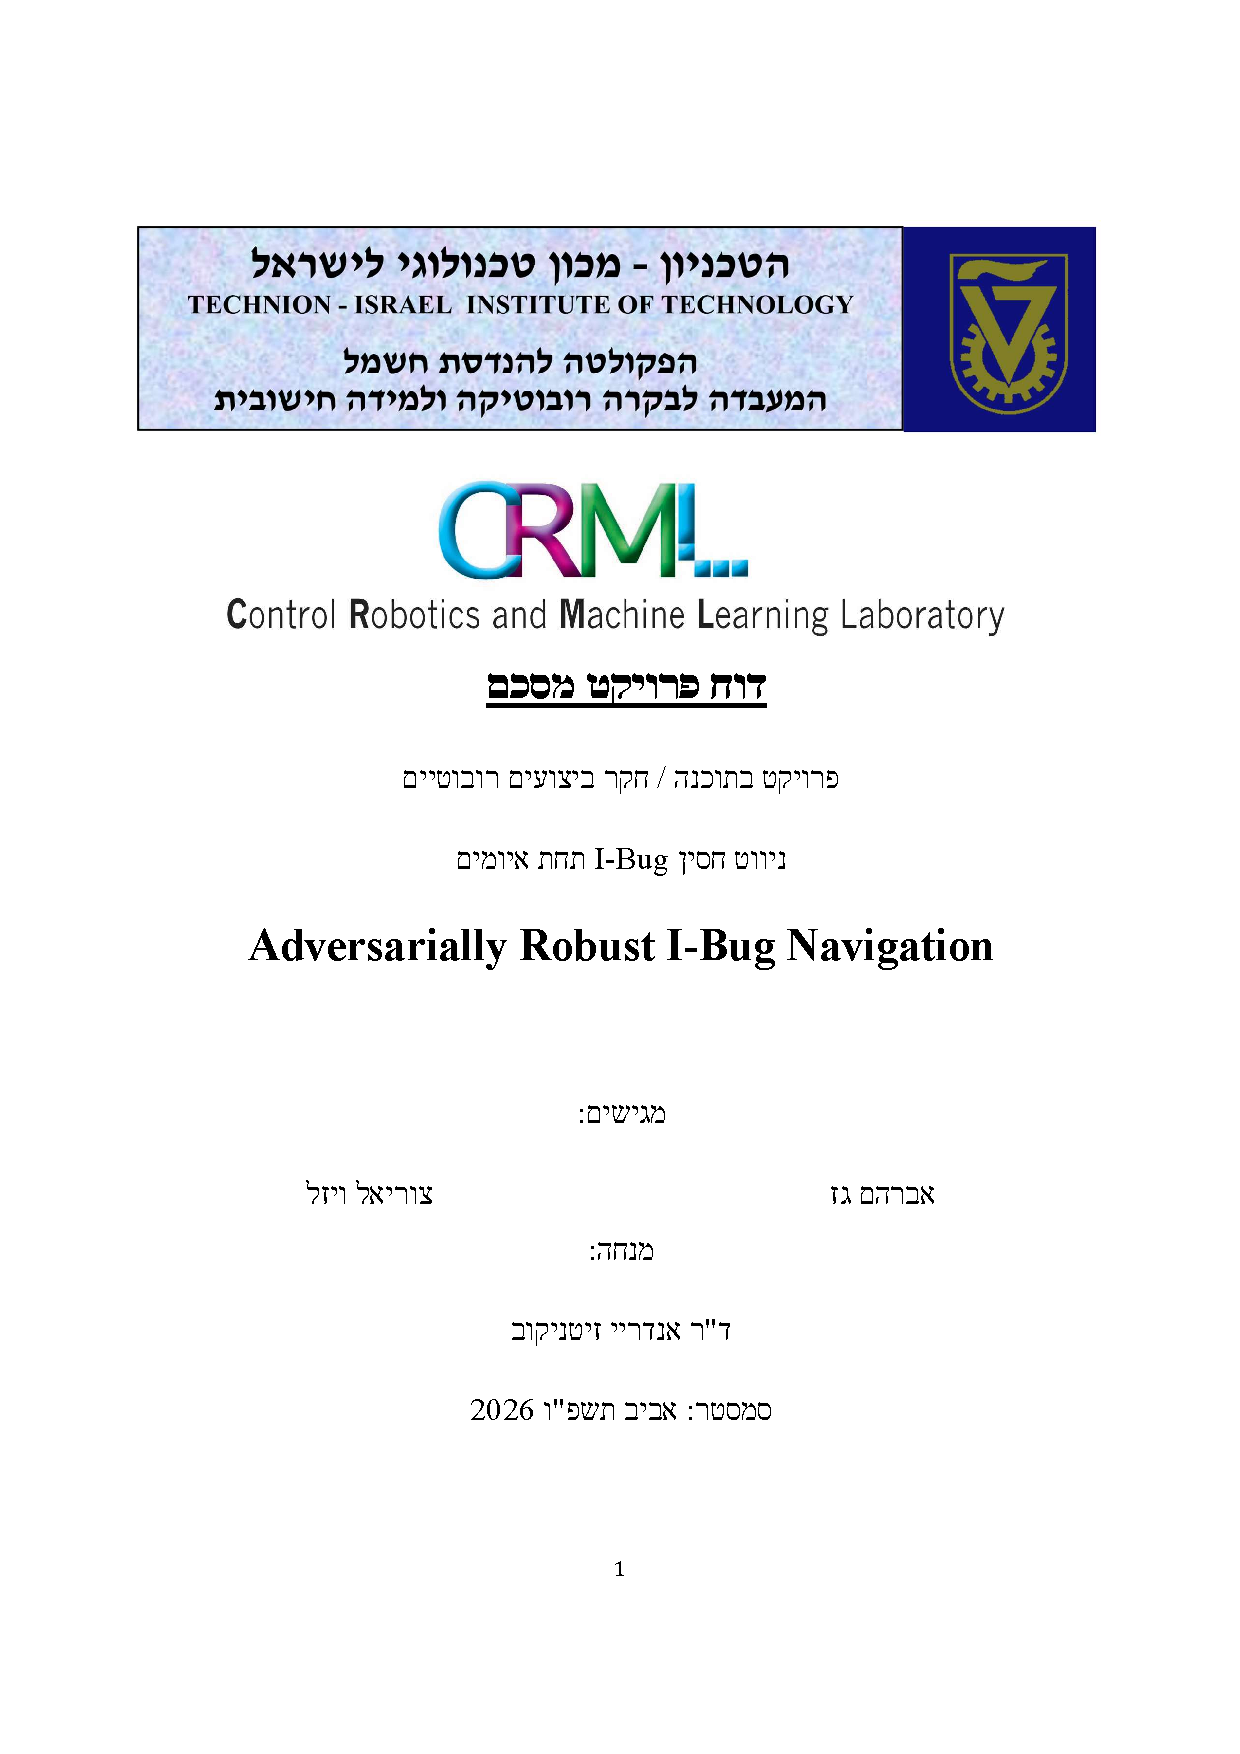
\includepdf[pages={1}]{titlepage.pdf}

% יצירת תוכן עניינים אוטומטי
% יצירת תוכן עניינים אוטומטי
\tableofcontents
\newpage

% יצירת רשימת איורים וטבלאות אוטומטית
\renewcommand{\listfigurename}{רשימת איורים}
\renewcommand{\listtablename}{רשימת טבלאות}
\listoffigures
\vspace{1.5cm} % מרווח אסתטי בין שתי הרשימות
\listoftables
\newpage

% ------------------- תקציר -------------------
\begin{abstract}
פרויקט זה מציג מחקר מעמיק ופיתוח של פתרונות ניווט עבור רובוטים מינימליסטיים הפועלים בסביבות בלתי מוכרות, ללא אמצעי לוקליזציה גלובליים (כגון \textenglish{GPS}) או מפות מוקדמות. העבודה נשענת על התשתית התיאורטית של אלגוריתם \textenglish{I-Bug}, אשר מאפשר הגעה ליעד תוך שימוש בחיישן מגע ובחיישן למדידת עוצמת אות (\textenglish{Intensity}) בלבד. הבעיה המרכזית שאותה תוקף פרויקט זה היא חוסר העמידות של אלגוריתמי הניווט הקלאסיים המבוססים על גרדיאנט-עוצמה מפני שיבושים מבוקרים – ספציפית, נוכחות של "מגדל פיראטי" (\textenglish{Adversarial transmitter}). תחת עקרון הסופרפוזיציה של גלים, המגדל הפיראטי משדר אותות כוזבים לסירוגין המתחברים לאות המקורי, מה שיוצר שיבושים מתמטיים בפונקציית העוצמה (פסגות שווא). כתוצאה מכך, האלגוריתם הקלאסי קורס, מאחר שהרובוט מקבל החלטות על בסיס נתונים מורעלים ונקלע ללולאות אינסופיות סביב מכשולים.

כדי להתמודד עם אתגר זה, פותח מנגנון זיהוי אנומליות המבוסס על חוסר רציפות (\textenglish{Discontinuity}) באות. על בסיס מנגנון זה, מומשו שתי אסטרטגיות בקרה חדשות הנשענות על ניהול חכם של מצב הזיכרון (\textenglish{State memory}) ללא צורך בחומרה נוספת: הגישה הזהירה (\textenglish{Cautious} - עצירה מוחלטת והקפאת זיכרון בעת שיבוש) והגישה האינרציאלית (\textenglish{Inertial} - המשך תנועה עיוורת מכוח האינרציה הלוגית תוך התעלמות מפסגות שווא).

במסגרת המתודולוגיה, פותחה סביבת סימולציה קינמטית רחבת-היקף בשפת \textenglish{Julia}. נותחו 1,000,000 סביבות אקראיות, כאשר כל סביבה נבחנה באופן השוואתי (\textenglish{Paired execution}) מול שלוש האסטרטגיות: הנאיבית (הקלאסית) ושתי האסטרטגיות החדשות. התוצאות מצביעות על כך שהבקר הנאיבי נכשל ב-42.57\% מהמקרים תחת איום (הצלחה של 57.43\% בלבד), מה שמוכיח את חומרת הבעיה המחקרית. מנגד, הבקר הזהיר (\textenglish{Cautious}) השיג שיעור הצלחה מוחלט של 100\%, תוך אימות ההוכחה המתמטית לשימור מסלול הניווט גם תחת סופרפוזיציה מלאה. הבקר האינרציאלי (\textenglish{Inertial}) רשם שיעור הצלחה של 99.11\%, כאשר כישלונותיו המעטים נבעו ממלכודות טופולוגיות נדירות של סנכרון מחזורי (\textenglish{Cyclic Synchronization}).

ניתוח התוצאות מצביע על \textenglish{Trade-off} מובהק בין בטיחות ליעילות תפעולית: בעוד שהבקר הזהיר מבטיח התכנסות מוחלטת אך דורש זמן ממושך יותר בגין השהיות (ממוצע של 189 צעדים למטרה), הבקר האינרציאלי מקצץ את משך הניווט משמעותית (ממוצע של 147.9 צעדים) ומציג שיפור יעילות של כ-21.7\%. הפרויקט מוכיח כי ניתן לחסן מערכות רובוטיות זולות מפני לוחמה אלקטרונית ושיבושי סביבה באמצעות אלגוריתמיקה חכמה, ומספק פלטפורמה לבחירה הנדסית בין בטיחות קשיחה למהירות אופטימלית.
\end{abstract}
\newpage

% ------------------- גוף הדוח -------------------

\section{מטרת הפרויקט והצגת הבעיה}

\subsection{רקע ומוטיבציה}
ניווט אוטונומי בסביבות לא מוכרות נשען לרוב על אמצעי חישה מתקדמים (כגון רדאר ו-\textenglish{LIDAR}) או על מערכות מיקום גלובליות (\textenglish{GPS}). עם זאת, בסביבות רבות (כגון חללים סגורים, אזורי אסון או שדות קרב משובשים) אמצעים אלו אינם זמינים, חושפים את המערכת לחסימות, או דורשים משאבי אנרגיה וחישוב שאינם מתאימים לפלטפורמות זעירות וזולות. 

גישת הרובוטיקה המינימליסטית, ובפרט משפחת אלגוריתמי הניווט מבוססי-החיישנים (\textenglish{Bug Algorithms}), נועדה לפתור בעיה זו. אלגוריתמים אלו מאפשרים ניווט מוכח ליעד באמצעות חישה מקומית בלבד, ללא הסתמכות על מפות מוקדמות. אלגוריתם \textenglish{I-Bug} מהווה מקרה קצה של גישה זו, שכן הוא דורש חיישן מגע למעקף מכשולים וחיישן למדידת עוצמת אות כיוונית בלבד, ללא דרישה לקואורדינטות מרחביות או למדידת מרחק אודומטרית.

\subsection{הגדרת הבעיה}
על אף האלגנטיות המתמטית של אלגוריתם \textenglish{I-Bug}, הוא מסתמך על הנחת יסוד מחמירה: מקור האות (מגדל המטרה) הוא יחיד, אמין ורציף. בפועל, גלים פיזיקליים (כגון גלי רדיו או אקוסטיקה) מצייתים לעקרון הסופרפוזיציה. 

בפרויקט זה מוגדר איום בדמות "מגדל פיראטי" (\textenglish{Adversarial transmitter}) המשדר אותות כוזבים לסירוגין. האותות הכוזבים מתחברים לאות המקורי ויוצרים שדה עוצמה משובש בעל "פסגות שווא" (\textenglish{False peaks}). כאשר הרובוט פועל תחת אלגוריתם קלאסי ומסתמך על מדידת הגרדיאנט לבדה, השיבושים הללו מרעילים את זיכרון המצבים של הבקר. כתוצאה מכך, קבלת ההחלטות משתבשת והרובוט נלכד בלולאות מעקב-גבולות אינסופיות סביב מכשולים, מבלי יכולת להגיע ליעד.

\subsection{יעדי הפרויקט}
מטרתו המרכזית של פרויקט זה היא להקנות חסינות (\textenglish{Adversarial Robustness}) לאלגוריתמי ניווט מבוססי-עוצמה מפני שיבושים אלקטרוניים, מבלי לפגוע בפרדיגמה המינימליסטית – קרי, ללא הוספת רכיבי חומרה לרובוט. לשם כך הוגדרו היעדים הבאים:
\begin{enumerate}
    \item \textbf{זיהוי האיום באופן אוטונומי:} אפיון ופיתוח פילטר מתמטי המסוגל להבחין בין שינוי גרדיאנט טבעי (הנובע מתנועת הרובוט) לבין קפיצה מלאכותית באות (הנובעת משיבוש), תוך התבססות על מגבלות הקינמטיקה.
    \item \textbf{פיתוח אסטרטגיות בקרה חסינות:} תכנון ומימוש אסטרטגיות ניווט חלופיות ברמת התוכנה לניהול זיכרון המצבים. בפרויקט נבחנו שתי אסטרטגיות: הגישה הזהירה (\textenglish{Cautious}) השואפת לבטיחות מוחלטת, והגישה האינרציאלית (\textenglish{Inertial}) השואפת למיקסום מהירות ההגעה.
    \item \textbf{אימות אמפירי והוכחה:} פיתוח סביבת סימולציה רציפה בשפת \textenglish{Julia} והרצת מערך ניסויים רחב-היקף (1,000,000 סביבות אקראיות) לכימות מדויק של ה-\textenglish{Trade-off} בין בטיחות ליעילות תפעולית.
\end{enumerate}


\section{מבוא ורקע תיאורטי מפורט}

\subsection{סקירת ספרות: מרובוטיקה קלאסית לניווט מינימליסטי}
תחום תכנון התנועה האוטונומית החל את דרכו עם מודלים שהניחו ידע גלובלי מוקדם על הסביבה. פריצת הדרך בתחום הניווט מבוסס-החיישנים התרחשה בעבודתם החלוצית של \textenglish{Lumelsky} ו-\textenglish{Stepanov} משנת 1987 \cite{lumelsky1987path}, אשר הציגו את אלגוריתמי ה-\textenglish{Bug} הראשונים. אלגוריתמים אלו הוכיחו כי רובוט נקודתי יכול להבטיח הגעה למטרה בסביבה מלאת מכשולים באמצעות חיישן מגע מקומי בלבד וידיעת קואורדינטות המטרה.

מאז, התפתחה משפחת אלגוריתמי ה-\textenglish{Bug} לשילוב חיישנים שונים לשם ייעול המסלול. דוגמה בולטת לכך היא אלגוריתם \textenglish{TangentBug} \cite{kamon1998tangentbug}, אשר עושה שימוש בחיישני טווח (כגון מד-טווח לייזר) כדי לקצר את נתיב ההליכה על ידי זיהוי מוקדם של פינות מכשולים. 

עם זאת, אלגוריתם \textenglish{I-Bug} לקח את המינימליזם הסנסורי לקצה. האלגוריתם הוצג לראשונה על ידי \textenglish{Taylor} ו-\textenglish{LaValle} בכנס \textenglish{ICRA} \cite{taylor2011ibug}, ובהמשך הורחב במאמר מקיף בכתב העת \textenglish{Autonomous Robots} בשנת 2014 \cite{taylor2014intensity}, אשר ביסס את ההוכחות המתמטיות להתכנסות גלובלית. בניגוד לקודמיו, \textenglish{I-Bug} אינו דורש לוקליזציה, אודומטריה או קואורדינטות. הוא מתבסס אך ורק על מדידת עוצמת אות המטרה לשם גזירת כיוון ומרחק יחסי.

\subsection{אלגוריתם \textenglish{I-Bug} ופעולות היסוד (\textenglish{Primitives})}
בבסיס האלגוריתם המקורי עומדת ההנחה כי קיימת פונקציית עוצמה חלקה ואנליטית, $m(p - p_t)$, העולה מונוטונית ככל שהמרחק הגיאומטרי למגדל המטרה $p_t$ מתקצר. הניווט מתבצע באמצעות מעברים לוגיים בין שלוש פעולות יסוד (\textenglish{Motion Primitives}):
\begin{enumerate}
    \item \textbf{התכווננות (\textenglish{Orient / $u_{ori}$}):} סריקה זוויתית למציאת כיוון הגרדיאנט התלול ביותר (הכיוון אל המטרה).
    \item \textbf{תנועה קדימה (\textenglish{Forward / $u_{fwd}$}):} תנועה בקו ישר לאורך הגרדיאנט, הנפסקת רק בהגעה למטרה או בהתנגשות במכשול.
    \item \textbf{מעקב גבולות (\textenglish{Follow / $u_{fol}$}):} הקפת מכשול תוך שמירת מגע. במהלך ההקפה, הרובוט דוגם את עוצמת האות כדי לאתר את הנקודה האופטימלית לעזיבת המכשול.
\end{enumerate}

\textbf{תנאי העזיבה (התקדמות מונוטונית):} 
הליבה המתמטית המבטיחה הגעה ליעד מבוססת על רישום העוצמה. כאשר הרובוט מתנגש במכשול, הוא שומר בזיכרון את העוצמה בנקודת הפגיעה ($i_H$). הרובוט מורשה לעזוב את המכשול (ולחזור לתנועה קדימה) אך ורק אם מצא לאורך הגבול נקודת מקסימום מקומי שבה העוצמה גדולה ממש מ-$i_H$. תנאי זה מבטיח כי כל עזיבה מתבצעת מנקודה קרובה יותר ליעד, מה שמונע כניסה ללולאות אינסופיות.

\subsection{תיאור הבעיה: מודל האיום וסופרפוזיציה}
המודל הקלאסי קורס כאשר למרחב מתווסף איום אלקטרומגנטי (מגדל פיראטי). פליטות פיזיקליות של גלי רדיו או קול מקיימות את עקרון הסופרפוזיציה. לכן, כאשר האויב משדר, האות הכולל הנקלט על ידי הרובוט, $S(p, t)$, אינו דורס את האות המקורי אלא מתווסף אליו:
\begin{equation}
S(p, t) = m(p - p_t) + e(t)
\end{equation}
כאשר $e(t) \ge 0$ מייצג את תוספת האות מהמגדל הפיראטי, הפועל לסירוגין. תוספת זו יוצרת פסגות שווא וגרדיאנטים מוטים. אם השיבוש מתרחש ברגע ההתנגשות במכשול, הרובוט אוגר בזיכרונו ערך $i_H$ שגוי וגבוה באופן מלאכותי. כשהמשדר הפיראטי נכבה, האות צונח בחזרה לערכו האמיתי, אך הבקר כבר "הורעל" ויישאר כלוא במעקב גבולות לנצח בניסיון למצוא ערך סף שאינו קיים פיזיקלית במציאות.

\subsection{אובדן רציפות כמנגנון זיהוי תקיפה}
על מנת להקנות לרובוט יכולת זיהוי אוטונומית של שיבושים ללא חומרה נוספת, פותח מנגנון אנומליות הנשען על עקרון הרציפות הקינמטית. 

רובוט הנע במרחב פועל תחת חסם מהירות עליון ($v_{max}$). מכיוון ששדה המטרה הטבעי $m$ הוא פונקציה רציפה (המקיימת את תנאי ליפשיץ עם קבוע $K$), הנגזרת הזמנית של האות הנקלט כתוצאה מתנועה בלבד חסומה תמיד על ידי: $\left| \frac{\partial m}{\partial t} \right| \le K \cdot v_{max}$.

לעומת זאת, הפעלה או כיבוי של המגדל הפיראטי מתנהגים כפונקציית מדרגה, היוצרת קפיצה (אובדן רציפות) כמעט מיידית במרחב הזמן, כך ש-$\frac{\partial S}{\partial t} \to \infty$. ההבחנה הברורה הזו מאפשרת לבקר להפריד באופן מתמטי בין שינוי עוצמה טבעי (גרדיאנט מרחבי) לבין התקפת סופרפוזיציה (אנומליה זמנית), ולהפעיל את אסטרטגיות הנגד שיפורטו בפרקים הבאים.



\section{תיאור מפורט - אסטרטגיות פתרון וניתוח \textenglish{Trade-offs}}
מתוך אפיון הבעיה והגדרת מנגנון זיהוי האנומליות (אובדן רציפות האות), גובשו ומומשו שלוש אסטרטגיות בקרה שונות. אסטרטגיות אלו מגדירות את תגובת הרובוט מרגע זיהוי ההתקפה, ומבוססות על ניהול שונה של זיכרון המצבים, ללא שינוי בחומרת המערכת.

\subsection{הבקר הנאיבי (\textenglish{Naive Baseline})}
הבקר הנאיבי מהווה את תצורת הבסיס לפרויקט, והוא מיישם את אלגוריתם ה-\textenglish{I-Bug} המקורי ללא כל מנגנון הגנה. תחת אסטרטגיה זו, מנגנון סינון האנומליות מנוטרל, והרובוט מתייחס לאות המורכב $S(p,t)$ כאילו היה הגרדיאנט האמיתי. הבקר מעדכן את זיכרון השיא המקומי ($i_H$) בצורה עיוורת גם כאשר קיימות פסגות שווא. בקר זה משמש כקבוצת ביקורת שנועדה לכמת את חומרת הבעיה ולהוות בסיס להשוואת ההתייעלות של האסטרטגיות האחרות.

\subsection{הבקר הזהיר (\textenglish{Cautious})}
אסטרטגיה זו תוכננה במטרה לשמור על אמינות הנתונים ועל הערובות התיאורטיות של האלגוריתם המקורי בכל מחיר. עם זיהוי אנומליה חיובית (קפיצה באות כתוצאה מהפעלת האויב), הבקר מכניס את הרובוט למצב 'השהיה' (\textenglish{Pause}):
\begin{itemize}
    \item \textbf{עצירה קינמטית:} מהירות הרובוט מאופסת מיידית ($\frac{dp}{dt} = 0$).
    \item \textbf{הקפאת זיכרון:} עדכון המשתנים הפנימיים, ובפרט זיכרון העוצמה המקסימלית $i_H$, מושעה לחלוטין.
    \item \textbf{מנגנון חזרה:} הרובוט ממתין במצב סטטי עד לזיהוי אנומליה שלילית (צניחה חדה באות המעידה על כיבוי המשדר הפיראטי). כדי לסנן רעשים, החזרה לתנועה מותנית בקבלת מספר דגימות רצופות ויציבות. לאחר אישור ניקיון האות, הרובוט ממשיך את פעולת היסוד (\textenglish{Primitive}) שהופסקה מאותה נקודה גיאומטרית מדויקת.
\end{itemize}
אסטרטגיה זו משמרת לחלוטין את המסלול הגיאומטרי האידיאלי, אך מטילה "קנס" של זמן פעולה ארוך עקב ההמתנה הסטטית.

\subsection{הבקר האינרציאלי (\textenglish{Inertial Heuristic})}
זוהי הגישה החדשנית ביותר שפותחה בפרויקט, המבוססת על המרת זמן השיבוש לזמן התקדמות מועיל, תחת ההנחה כי מערכת הנמצאת בתנועה יכולה להפיק תועלת מהמשך התנועה בחוג פתוח (\textenglish{Open-loop}).
כאשר הבקר האינרציאלי מזהה אנומליה, הוא מקפיא את כתיבת הנתונים לזיכרון ה-$i_H$ (כדי למנוע הרעלה), אך במקום לעצור את התנועה המרחבית, הוא מקפיא את זווית ההתקדמות וממשיך לנוע מכוח האינרציה הלוגית:
\begin{itemize}
    \item אם הרובוט פעל במצב התקדמות ליעד ($u_{fwd}$), הוא ימשיך לנוע בקו ישר (עיוור). 
    \item אם במהלך התנועה העיוורת הרובוט מתנגש במכשול, הוא יוזם מעקב גבולות ($u_{fol}$) תוך שימוש בערך האות התקין האחרון שנשמר לפני תחילת השיבוש.
    \item במהלך מעקב גבולות תחת שיבוש, הרובוט משעה את תנאי העזיבה (חיפוש מקסימום מקומי), מאחר שהקריאות הנוכחיות מוטות. הוא מחפש נקודת עזיבה רק לאחר שהאות חוזר ליציבות.
\end{itemize}
אסטרטגיה זו מאפשרת ניווט רציף ומהיר במיוחד, אך מתפשרת על הבטחת ההגעה התיאורטית, שכן התנועה העיוורת עלולה להוביל לפספוס נקודות עזיבה קריטיות.

\subsection{סיכום ה-\textenglish{Trade-offs}}
ליבת הפרויקט מציגה דילמה הנדסית קלאסית: בחירה בין בטיחות קשיחה ליעילות תפעולית. בעוד שהבקר הנאיבי כושל לחלוטין, הבקר הזהיר מקריב יעילות זמן למען הבטחת הגעה גלובלית. מנגד, הבקר האינרציאלי מתפקד כהיוריסטיקה חכמה – הוא מגן על הזיכרון במקביל לניצול הדינמיקה המכנית כדי לחסוך זמן משמעותי, אך לוקח סיכון מחושב של הילכדות סביב מכשולים מורכבים מבחינה טופולוגית.

\section{הוכחה מתמטית: ערובות התכנסות של הבקר הזהיר}
ייחודו של הבקר הזהיר (\textenglish{Cautious}) טמון בכך שהוא האסטרטגיה היחידה מבין השלוש המספקת ערובה מתמטית קשיחה (\textenglish{Guarantee}) להגעה ליעד, תוך שימור מלא של תכונות המסלול המקוריות של אלגוריתם ה-\textenglish{I-Bug}, אפילו תחת סופרפוזיציה מלאה של אותות שיבוש.

\begin{theorem}[שימור מסלול מרחבי והתכנסות]
תחת הנחות רציפות המרחב (סעיף 2.4) ועקרון הסופרפוזיציה (סעיף 2.3), רובוט המיישם את אסטרטגיית "הבקר הזהיר" יגיע למגדל המטרה במספר סופי של צעדים מרחביים, בהינתן שקיים מסלול חוקי. העקבה הגיאומטרית (המסלול המרחבי) שיעבור הרובוט זהה לחלוטין למסלול שהיה עובר בסביבה סטרילית ונקייה משיבושים. כפועל יוצא, החסם העליון על המרחק הכולל זהה לזה של אלגוריתם \textenglish{I-Bug} המקורי, בעוד שזמן הביצוע הכולל גדל ליניארית ביחס למשך הזמן המצטבר שבו פעל משדר האויב.
\end{theorem}

\begin{proof}
בפרקי זמן שבהם האות תקין (היעדר אנומליה), הרובוט פועל בדיוק על פי פעולות היסוד וכללי מעבר המצבים (\textenglish{State-transition rules}) של אלגוריתם ה-\textenglish{I-Bug} המקורי.

כאשר המשדר העוין מופעל, הרובוט מזהה את אי-הרציפות בזמן שנוצרה כתוצאה מתוספת האות $e(t)$, ופוקד באופן מיידי על מהירות אפס ($\frac{dp}{dt} = 0$). עצירה זו נועלת את קואורדינטות המרחב של הרובוט $q = (x, y, \theta)$ ומשעה לחלוטין כל עדכון בזיכרון המצבים הפנימי (ובפרט את $i_H$ ואת מעקב המקסימום המקומי).

מכיוון שהמהירות המרחבית היא אפס מוחלט, מצב הרובוט נותר סטטי לחלוטין למשך כל זמן פעולת המשדר העוין. תוספת האות $e(t)$ אמנם משבשת את קריאת החיישן, אך אין לה כל השפעה על לוגיקת הבקרה שהוקפאה. כאשר האויב מכבה את השידור, $e(t)$ צונח חזרה לאפס, מה שמעורר אנומליה שלילית המאשרת כי הסביבה נקייה. קריאת החיישן חוזרת באופן מיידי לשקף את הגרדיאנט המרחבי האמיתי $m(p - p_t)$.

בנקודה זו, הרובוט מחדש את פעולות היסוד מאותן קואורדינטות מרחביות ומאותו מצב פנימי בדיוק בו היה טרם השיבוש. לפיכך, העקבה המרחבית $\gamma_{cautious}$ שעובר הרובוט חופפת בשלמותה למסלול התיאורטי $\gamma_{ideal}$ ללא הפרעות. 

הלכה למעשה, על ידי עצירת התנועה הקינמטית, הבקר "מוחק" את פרקי הזמן המושחתים מתוך ציר הזמן המקומי של הרובוט. טרנספורמציה זו של קיצוץ זמני השיבוש ממפה את הבעיה בחזרה ובאופן מושלם לבעיית הניווט הסטנדרטית שהוגדרה על ידי \textenglish{Taylor} ו-\textenglish{LaValle} \cite{taylor2014intensity}. מכיוון שבעבודתם המקורית סופקה הוכחה פורמלית להתכנסות מסלול זה במרחק סופי, הבקר הזהיר יורש את ערובת ההתכנסות הזו במלואה. "הקנס" היחיד שנוסף למערכת הוא הזמן המצטבר של תקופות ההשהיה.
\end{proof}

בעוד שהבקר הזהיר מעניק ערובה תיאורטית חזקה זו, הבקר האינרציאלי חסר אותה מיסודו. על ידי המשך תנועה דינמית עיוורת תוך כדי שיבוש, מסלולו חורג מ-$\gamma_{ideal}$. חריגה זו עלולה לגרום לרובוט לעקוף פיזית את נקודות העזיבה האופטימליות, מה שמפר את תנאי הסיום התיאורטיים של מעקב הגבולות ומייצר סיכון להילכדות בלולאות מחזוריות (כפי שהוכח אמפירית בסימולציה).

\section{תיאור תוכנה ומתודולוגיית סימולציה}
על מנת לתקף את המודלים התיאורטיים ולבחון את האסטרטגיות שהוצעו תחת תנאי קצה, פותחה פלטפורמת סימולציה קינמטית דו-ממדית בשפת \textenglish{Julia}. הסימולציה נמנעה משימוש ברשתות גריד בדידות ומימשה רזולוציה מרחבית רציפה, תוך הדמיית התנגשויות נוקשות ושדות אות דינמיים.

\subsection{המודל הקינמטי ותבנית האיום}
תנועת הרובוט מומשה במערכת קואורדינטות רציפה, כאשר לרובוט הוגדר רדיוס התנגשות פיזי וטווח חיישן מגע מקומי. פונקציית האות המקורי חושבה כהופכי של המרחק האוקלידי למגדל המטרה ($1/d$). מגדל האויב פעל תחת מחזור פעילות (\textenglish{Duty Cycle}) קבוע של 25\% (פעיל ל-10 צעדים, כבוי ל-30 צעדים), תוך פליטת אות כוזב קבוע שהתחבר בסופרפוזיציה לעוצמת האות האמיתית.
כדי להבטיח בקרת ניסוי קפדנית, יושמה מתודולוגיה של ביצוע מוצמד (\textenglish{Paired Evaluation}): עבור כל סביבה שנוצרה, שלושת הרובוטים (הנאיבי, הזהיר והאינרציאלי) חוו בדיוק את אותם תנאים טופולוגיים ותזמוני ל"א זהים, כשהם יוצאים מאותה נקודת התחלה.

\subsection{מחולל סביבות טופולוגיות}
בחינת אלגוריתמי ניווט דורשת יצירת מבוכים מורכבים מבחינה טופולוגית, אך פתירים מתמטית. לשם כך, פותח מחולל פרוצדורלי שייצר סביבות שטח בגודל $20 \times 20$ יחידות. כל סביבה אוכלסה ב-10 עד 16 מכשולים מלבניים. 
בכדי לאפשר יצירת מבנים מורכבים (כגון צורות U או מסדרונות ללא מוצא), מחולל המפות התיר חפיפה ומיזוג של מכשולים. יחד עם זאת, נאכפו שני חוקים גיאומטריים נוקשים למניעת סביבות בלתי-עבירות:
\begin{enumerate}
    \item \textbf{מניעת מעברים צרים (\textenglish{Narrow Gap Prevention}):} המרחק המרחבי בין כל שני מכשולים נפרדים אולץ להיות גדול מקוטרו הפיזי של הרובוט.
    \item \textbf{שולי המערכת (\textenglish{Perimeter Margin}):} כלל המכשולים הוגבלו במרחק ביטחון מגבולות הזירה, מה שהבטיח קיומו של נתיב היקפי פתוח תמיד, גם במקרה של צפיפות קיצונית במרכז המפה.
\end{enumerate}

\subsection{היקף הניסוי והרצות אצווה (\textenglish{Batch Processing})}
כדי לבסס מובהקות סטטיסטית ולכדוד מקרי קצה נדירים, הוגדרה מערכת הרצות אצווה ללא ממשק גרפי (\textenglish{Headless simulation}). המערכת הגרילה ופתרה 1,000,000 סביבות ייחודיות. עבור כל הרצה, הוגדר תקציב של 600 צעדים למשימה; חריגה מהתקציב או הילכדות בלולאה אינסופית סווגו ככישלון. התוצאות, לרבות זמני ההגעה, מצב ההצלחה והמסלולים, נשמרו לקבצי \textenglish{CSV} מרוכזים לשם ניתוח הנתונים והפקת הגרפים להלן.

\section{תוצאות ומדדים}
כדי להעריך את היעילות, הבטיחות וזמני ההתכנסות של האסטרטגיות השונות תחת איום סופרפוזיציה, נותחו התוצאות מתוך 1,000,000 הרצות הסימולציה. הנתונים מאמתים באופן מובהק את הפערים התיאורטיים שהוצגו בפרקים הקודמים, ומצביעים על דילמה תפעולית ברורה.

\subsection{אחוזי הצלחה ואמינות הניווט (\textenglish{Reliability})}
ניתוח שיעורי ההצלחה (איור \ref{fig:success_rates}) ממחיש את הקריסה המוחלטת של מודל הניווט הקלאסי תחת איום ל"א מתמשך. הבקר הנאיבי נכשל ב-42.57\% מהמקרים (שיעור הצלחה של 57.43\% בלבד). כישלונות אלו נבעו מהרעלת זיכרון ה-$i_H$ בעת פגיעה במכשולים, אשר הובילה את הרובוט ללולאות אינסופיות סביב גבולות המכשול בהמתנה לערך סף בלתי אפשרי.

\begin{figure}[htbp]
    \centering
    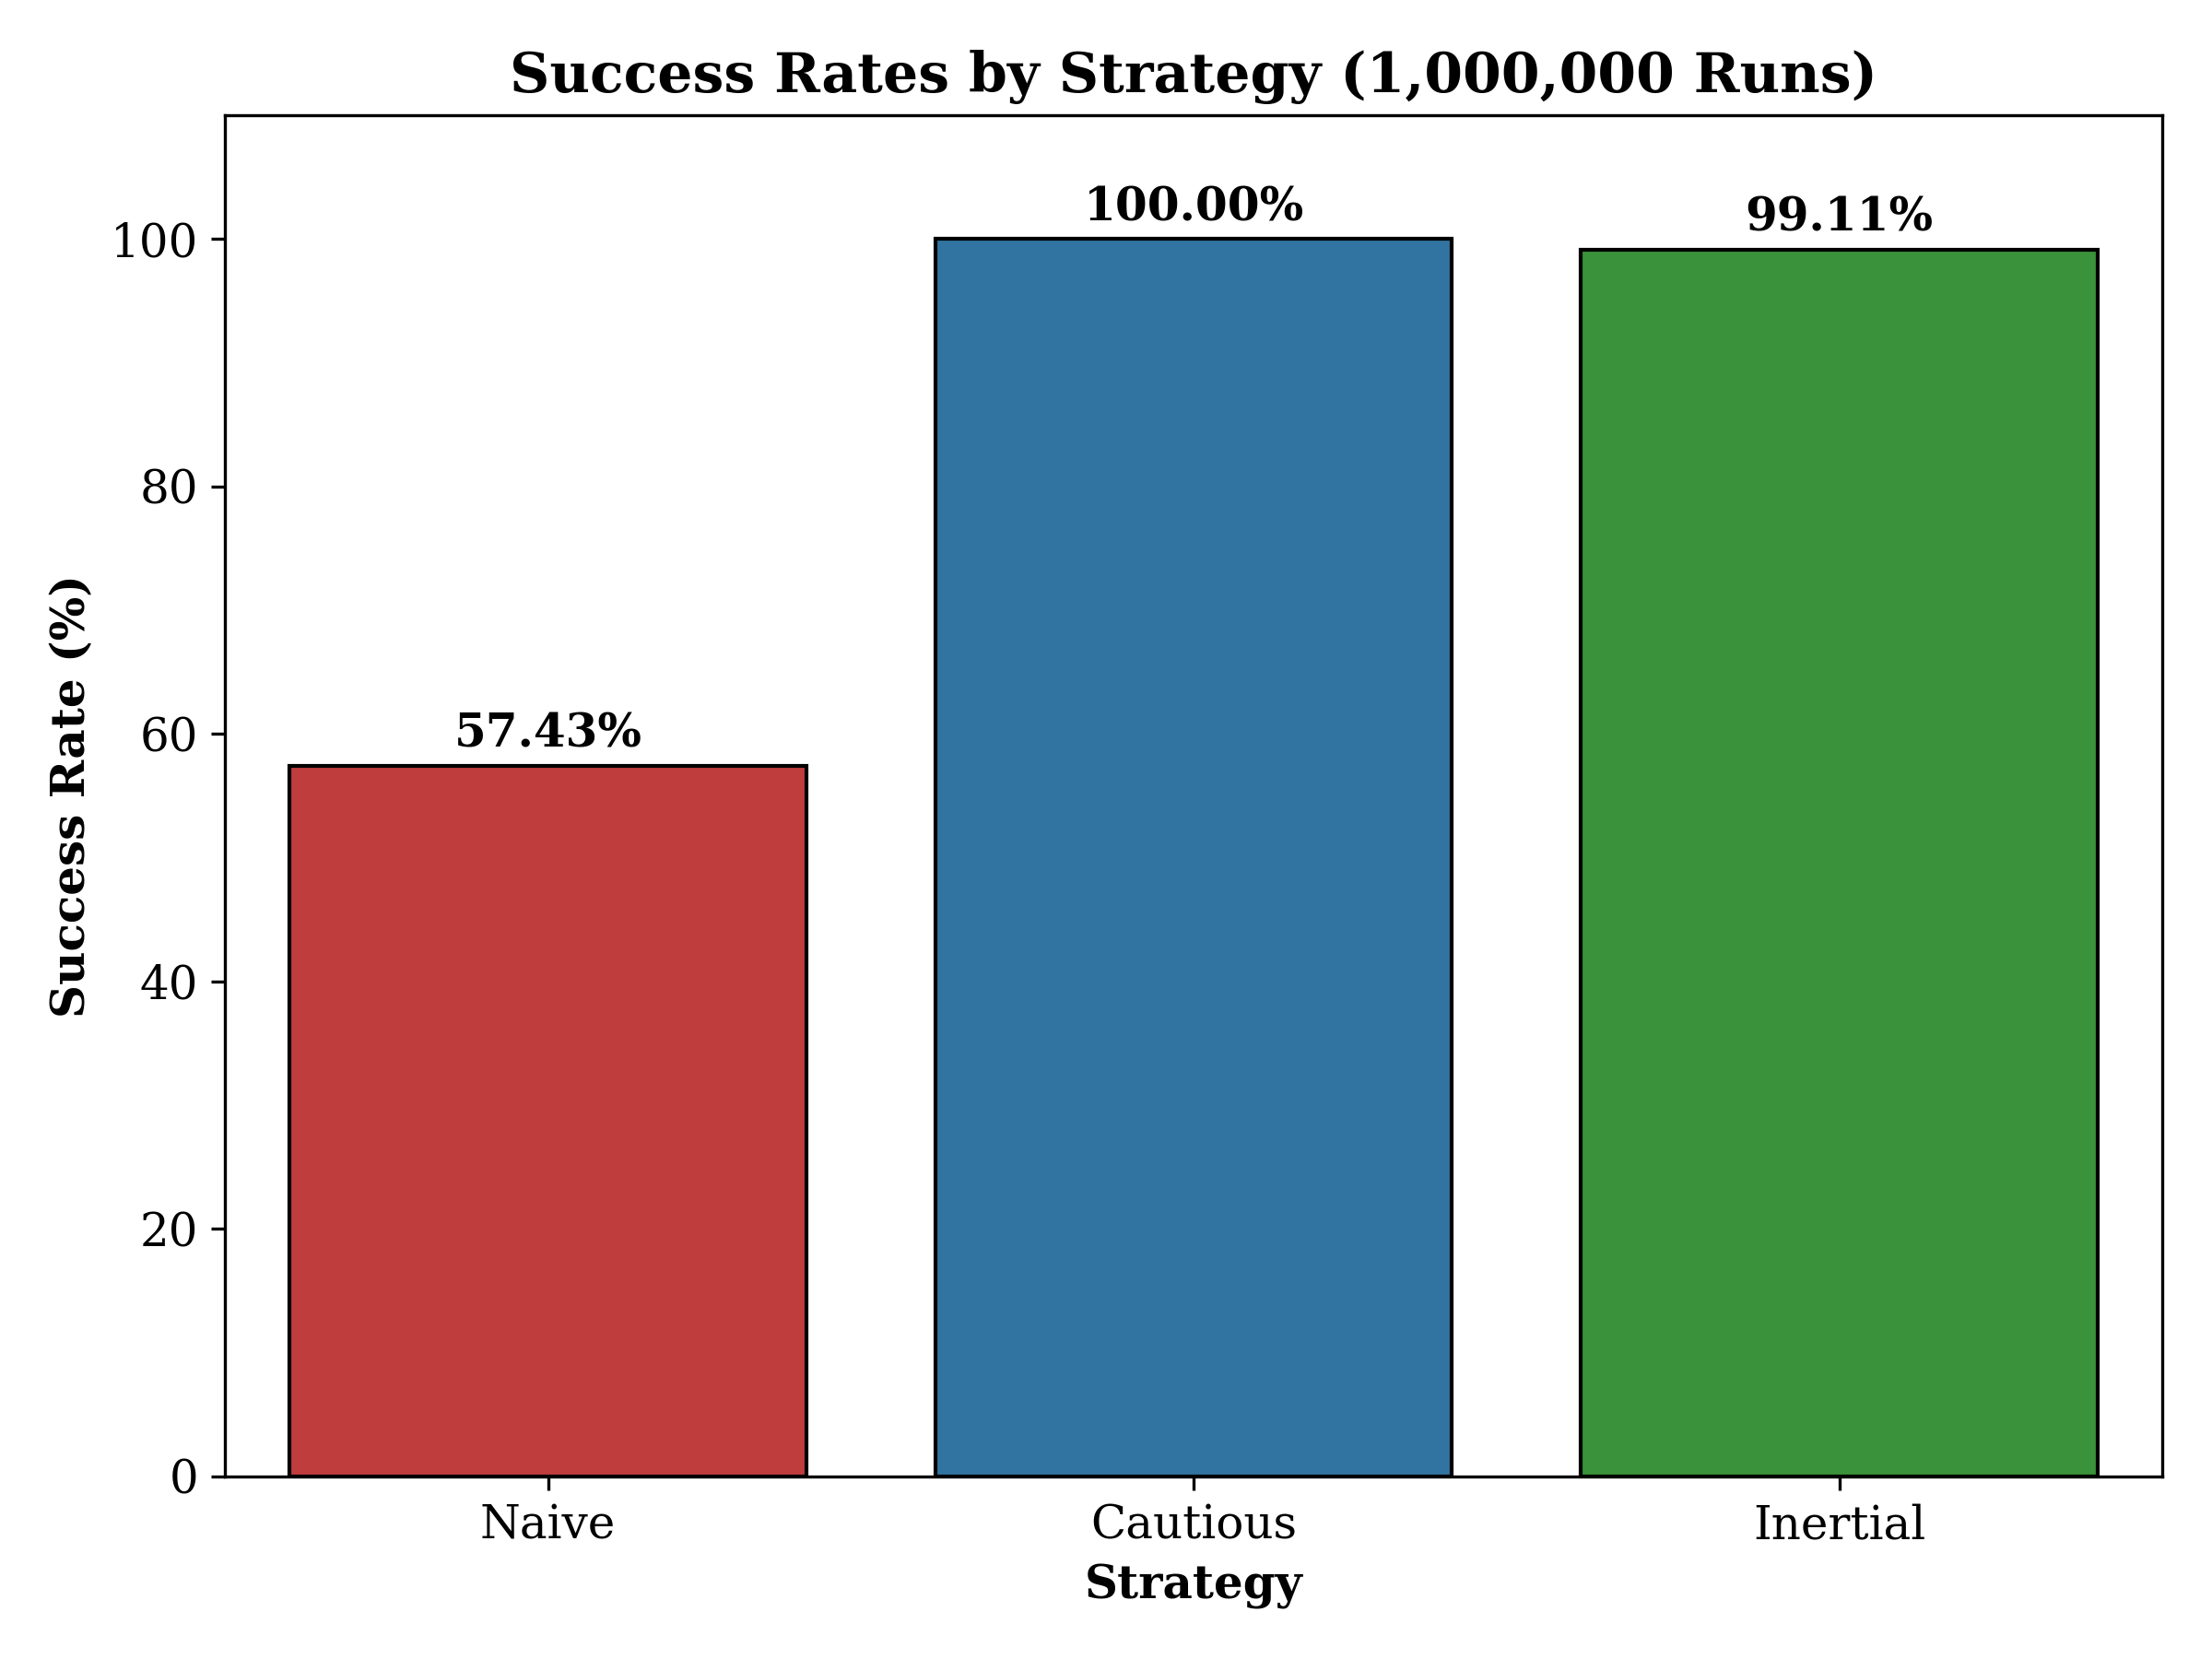
\includegraphics[width=0.9\linewidth]{success_rates.png}
    \caption{שיעורי ההצלחה של שלוש האסטרטגיות (הנאיבית, הזהירה והאינרציאלית) מתוך 1,000,000 סביבות אקראיות נגועות בשיבוש.}
    \label{fig:success_rates}
\end{figure}

לעומתו, אסטרטגיות ניהול הזיכרון תיקנו את הכשל התיאורטי כמעט לחלוטין. הבקר הזהיר (\textenglish{Cautious}) השיג שיעור הצלחה מוחלט של 100.00\%. נתון אמפירי זה מאשרר את ההוכחה המתמטית: הקפאת הקינמטיקה וזיכרון המצבים בזמן שיבוש משמרת את מסלול ההתקדמות הגיאומטרי המקורי ומונעת סטייה מהגבולות התיאורטיים של האלגוריתם. 

הבקר האינרציאלי (\textenglish{Inertial}) הפגין ביצועים מעולים כהיוריסטיקה, עם שיעור הצלחה של 99.11\%. כישלונו ב-0.89\% ממקרי הקצה מאשש את החולשה התיאורטית שלו: תנועה עיוורת ללא חיפוש מקסימום מקומי עלולה להוביל, בהסתברות נמוכה, לפספוס נקודות עזיבה וללכידה במלכודות טופולוגיות.

\subsection{יעילות מרחבית וזמני הגעה (\textenglish{Efficiency})}
ה-\textenglish{Trade-off} ההנדסי המרכזי של הפרויקט נחשף בניתוח כמות הצעדים הנדרשת להשלמת הניווט (איור \ref{fig:steps_dist} וטבלה \ref{tab:efficiency}). הנתונים חושבו אך ורק מתוך הרצות שהסתיימו בהצלחה.

הבקר הזהיר מבטיח אמנם הצלחה מוחלטת, אך גובה "קנס" תפעולי כבד עקב זמני ההמתנה בהם הרובוט קפוא במקומו. כתוצאה מכך, הוא דורש בממוצע 189.0 צעדים למטרה. מנגד, הבקר האינרציאלי, המנצל את זמן השיבוש להתקדמות קינמטית גיאומטרית, חוסך זמן משמעותי ומסיים את המסלול בממוצע של 147.9 צעדים.

\begin{table}[htbp]
\centering
\caption{השוואת יעילות ניווט תחת איום (ממוצע מתוך 1,000,000 הרצות)}
\label{tab:efficiency}
\begin{tabular}{@{}lcc@{}}
\toprule
\textbf{אסטרטגיה} & \textbf{שיעור הצלחה (\%)} & \textbf{ממוצע צעדים (בהרצות מוצלחות)} \\ \midrule
הבקר הנאיבי             & 57.43\%                    & 169.7                                \\
הבקר הזהיר          & 100.00\%                   & 189.0                                \\
הבקר האינרציאלי          & 99.11\%                    & 147.9                                \\ \bottomrule
\end{tabular}
\end{table}

\begin{figure}[htbp]
    \centering
    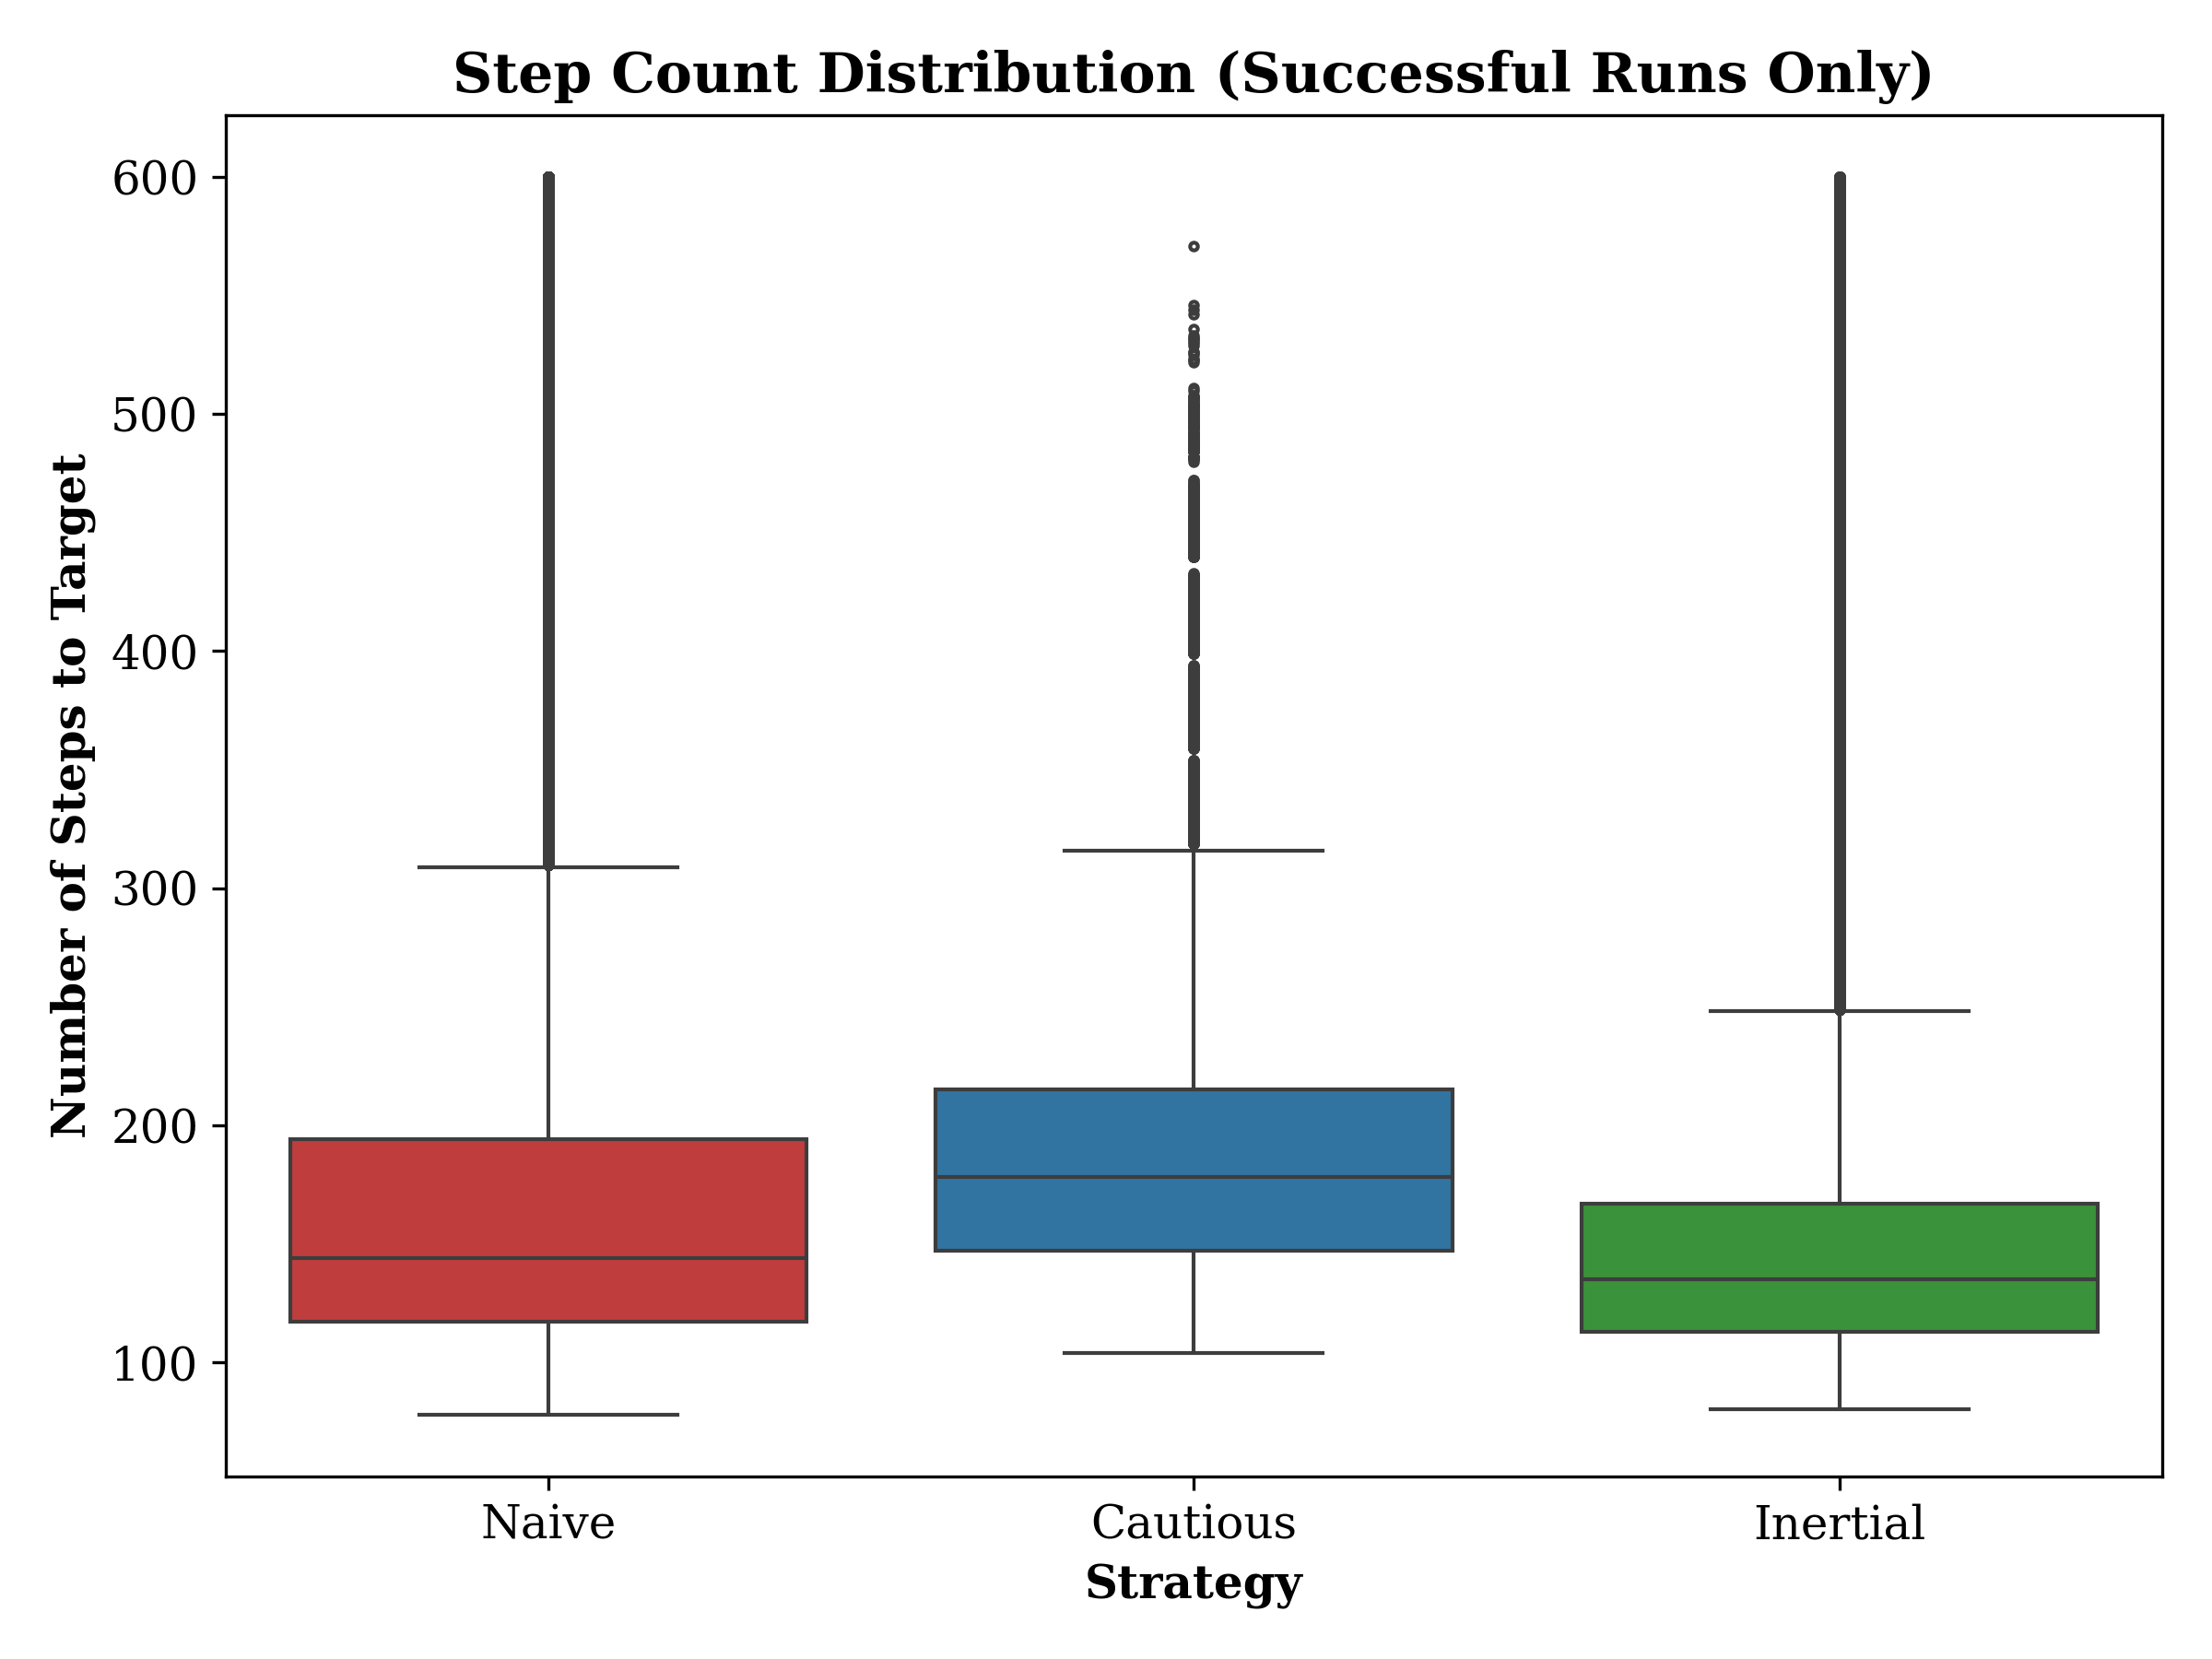
\includegraphics[width=0.9\linewidth]{steps_distribution.png}
    \caption{התפלגות כמות הצעדים הנדרשת להגעה למטרה בהרצות מוצלחות. הפיזור הגבוה של הבקר הזהיר מצביע על העלות הטמפורלית של ההמתנה.}
    \label{fig:steps_dist}
\end{figure}

פער זה מציג שיפור יעילות של כ-21.7\% לטובת המודל האינרציאלי, ומגדיר פרדיגמת תכנון עתידית: בחירה במודל הזהיר כאשר מחיר הטעות (כישלון בניווט) הוא אנוש, ובחירה במודל האינרציאלי כאשר המערכת נדרשת למקסם מהירות ומסוגלת לסבול שיעור כשל מזערי.

\subsection{הוכחה ויזואלית: סנכרון מחזורי (\textenglish{Cyclic Synchronization})}
במסגרת הסימולציה נצפו אותם 0.89\% של מקרי קצה שהובילו לכישלון הבקר האינרציאלי. איור \ref{fig:sim_trap} מציג תיעוד מתוך סביבת הסימולציה הממחיש את מלכודת הסנכרון המחזורי. ניתן לראות כיצד הרובוט האינרציאלי (בירוק) נקלע ללולאת הקפה עיוורת סביב המכשול עקב היעדר אימות של פונקציית המקסימום המקומי, בעוד שהרובוט הזהיר (בכתום) שורד את השיבוש ומגיע ליעדו.

\begin{figure}[htbp]
    \centering
    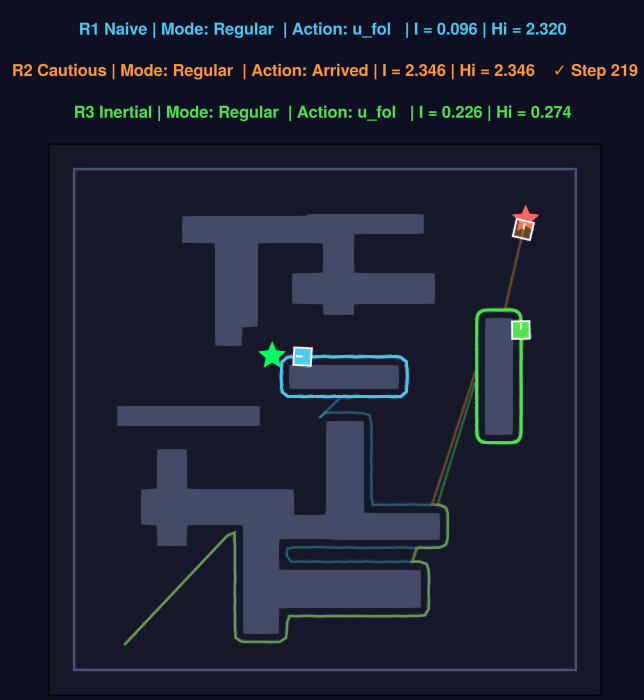
\includegraphics[width=0.8\linewidth]{simulation_trap.png}
    \caption{המחשה ויזואלית של מלכודת סנכרון מחזורי מתוך הסימולציה. הרובוט האינרציאלי (בירוק) כלוא בלולאת מעקב-גבולות אינסופית כתוצאה מתנועה עיוורת, בעוד הרובוט הזהיר (בכתום) מגיע ליעדו הודות להקפאת התנועה.}
    \label{fig:sim_trap}
\end{figure}


\section{סיכום ומסקנות}
מטרתו של פרויקט זה הייתה לבסס חסינות אלגוריתמית (\textenglish{Adversarial Robustness}) עבור רובוטים בעלי חישה מינימלית הפועלים במרחב אלקטרומגנטי עוין. המחקר הוכיח כי אלגוריתמי ניווט קלאסיים מבוססי-עוצמה (כדוגמת \textenglish{I-Bug}) קורסים לחלוטין כאשר סביבתם מופרעת על ידי שידורי סופרפוזיציה.

התרומה המרכזית של פרויקט זה היא בפיתוח מתודולוגיה המייתרת את הצורך בחומרה נוספת לשם התגוננות. באמצעות יישום פילטר אנומליות הנשען על עקרון הרציפות המרחבית, הודגם כיצד ניתן לחלץ סמנים זמניים (\textenglish{Temporal cues}) מתוך מידע מרחבי כוזב. על בסיס זיהוי זה, פותחו שתי אסטרטגיות המנהלות את זיכרון המצבים של הבקר.

התוצאות האמפיריות מתוך 1,000,000 הרצות סימולציה הצביעו על מסקנות חד-משמעיות:
\begin{itemize}
    \item \textbf{בטיחות מתמטית מוחלטת:} הבקר הזהיר מבטיח 100\% התכנסות ליעד. הקפאת הקינמטיקה מבטלת כליל את ההשפעה של שדה עוצמה משובש ומונעת הרעלת זיכרון.
    \item \textbf{יעילות תפעולית תחת סיכון מחושב:} הבקר האינרציאלי מספק אמינות כמעט מוחלטת (99.11\%) תוך קיצוץ מסיבי של זמני הניווט (שיפור של כ-21.7\% ביעילות). 
\end{itemize}

מסקנות אלו מאפשרות למתכנני מערכות רובוטיות זולות להתאים את אלגוריתם הניווט לדרישות המשימה: בחירה בהשהיה בטוחה במשימות קריטיות, או בחירה בתנועה אינרציאלית רציפה ביישומי זמן-אמת (\textenglish{Real-time}). 

עבודה עתידית בנושא עשויה לכלול פיתוח של מנגנוני שבירת-תהודה סטוכסטיים (\textenglish{Stochastic Resonance Breaking}) – כלומר, הוספת רעש אקראי לתנועת הבקר האינרציאלי במטרה לחלץ אותו מטופולוגיות מחזוריות מבלי לפגוע ביעילותו. בנוסף, בדומה לאופן שבו אלגוריתם ה-\textenglish{I-Bug} המקורי אומת על גבי פלטפורמת רובוטיקה פיזית בסיסית \cite{taylor2014intensity}, מומלץ לבחון את המודלים החסינים שפותחו בפרויקט זה על גבי פלטפורמה רובוטית פיזית תחת תנאי לוחמה אלקטרונית ושיבושי ערוץ בעולם האמיתי.
\newpage
% ------------------- ביבליוגרפיה -------------------
\renewcommand{\refname}{רשימת מקורות}
\begin{thebibliography}{9}

\bibitem{lumelsky1987path}
\textenglish{V. J. Lumelsky and A. A. Stepanov, ``Path-planning strategies for a point mobile automaton moving amidst unknown obstacles of arbitrary shape,'' \textit{Algorithmica}, vol. 2, no. 1, pp. 403--430, 1987.}

\bibitem{kamon1998tangentbug}
\textenglish{I. Kamon, E. Rivlin, and E. Rimon, ``A new range-sensor based universally convergent obstacle avoidance algorithm,'' \textit{IEEE Trans. Robot. Autom.}, vol. 14, no. 2, pp. 227--233, Apr. 1998.}

\bibitem{taylor2011ibug}
\textenglish{K. Taylor and S. M. LaValle, ``I-Bug: An intensity-based bug algorithm,'' in \textit{Proc. IEEE Int. Conf. Robot. Autom. (ICRA)}, Shanghai, China, 2011, pp. 3981--3986.}

\bibitem{taylor2014intensity}
\textenglish{K. Taylor and S. M. LaValle, ``Intensity-based navigation with global guarantees,'' \textit{Autonomous Robots}, vol. 36, no. 4, pp. 349--364, 2014.}

\end{thebibliography}

\end{document}